\documentclass[../main.tex]{subfiles}
\begin{document}
\chapter{Tecniche di microscopia a super-risoluzione}

\section{Microscopi ottici}

I primi microscopi furono costruiti nel 17\textdegree\ secolo, oltre 400 anni fa e furono utilizzati per vedere per la prima volta i microrganismi che abitano la Terra. In quest'epoca ebbe inizio lo studio della \gls{microbiologia}. Lo studioso \textit{Robert Hooke} osservò le pareti cellulari e usò per la prima volta il termine ``cellula" \cite{fara_2009, micrographia}. Nel 1663 \textit{Antoine van Leeuwenhoek} fabbricò artigianalmente dei microscopi semplici, a singola lente, con ingrandimenti molto superiori rispetto a quelli esistenti a quell'epoca e fu il primo ad osservare microrganismi, come batteri, protozoi e globuli rossi.\cite{lane_2015, dobell_1923, corliss_1975, jessup_2024}

Il microscopio ottico composto ingrandisce l'immagine del campione usando due o più lenti. Il campione viene illuminato usanto una sorgente di luce sul lato opposto all'obiettivo (microscopia a luce trasmessa) oppure sullo stesso lato (microscopia a luce riflessa).

Il sistema più semplice è composto da due lenti, una lente obiettivo vicina al campione da esaminare, e una lente oculare vicina all'osservatore. Il campione è prima messo a fuoco dalla lente obiettivo dentro al microscopio in un'immagine reale, che è creata dalla convergenza dei raggi di luce, poi questa immagine viene nuovamente ingrandita dalla lente oculare che crea una immagine virtuale, generata dalle proiezioni di raggi divergenti. L'osservatore quindi vede un'immagine ingrandita, invertita e virtuale del campione esaminato.

\begin{figure}[h]
\centering
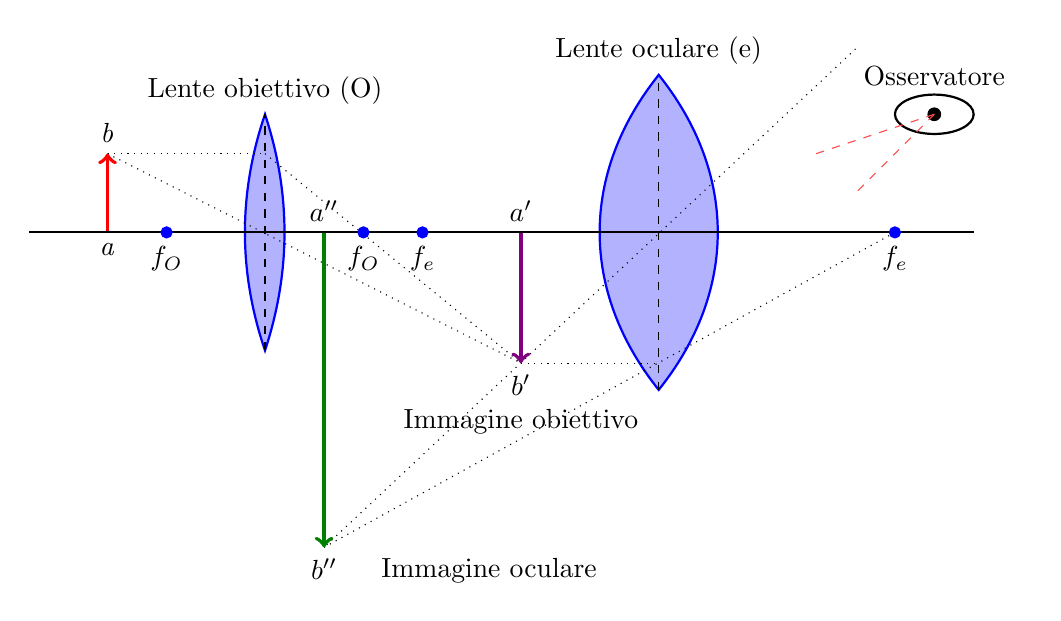
\begin{tikzpicture}
	% lente obiettivo
	\filldraw[thick,blue!30, draw=blue] (3,1.5)
		.. controls (2.66,0.5) and (2.66,-0.5) .. (3,-1.5)
		.. controls (3.33,-0.5) and (3.33,0.5) .. cycle
		node[black,above] {Lente obiettivo (O)};
	\draw[dashed] (3,-1.5) -- (3,1.5);

	% lente oculare
	\filldraw[thick,blue!30, draw=blue] (8,2)
	.. controls (9,0.75) and (9,-0.75) .. (8,-2)
	.. controls (7,-0.75) and (7,0.75) .. cycle
	node[black,above] {Lente oculare (e)};
	\draw[dashed] (8,-2) -- (8,2);

	\draw[dotted] (1,1) -- (3,1);
	\draw[dotted] (3,1) -- (6.25,-1.66);
	\draw[dotted] (1,1) -- (6.25,-1.66);

	\draw[dotted] (6.25,-1.66) -- (8,-1.66);
	\draw[dotted] (11,0) -- (3.75,-4);
	\draw[dotted] (10.5,2.33) -- (3.75,-4);

	% oggetto
	\draw[line width=0.5mm,Red,->] (1,0) node[below, black] {\textit{a}}
		-- (1,1) node[above, black] {\textit{b}};

	% immagine reale
	\draw[line width=0.5mm,Purple,->] (6.25,0) node[above, black] {$a'$}
		-- (6.25,-1.66) node[below, black, align=center] {$b'$ \\ \text{Immagine obiettivo}};

	% immagine virtuale
	\draw[line width=0.5mm,Green,->] (3.75,0) node[above, black] {$a''$}
		-- (3.75,-4) node[below, black] {$b''$} node[below right, black] {\ \ \quad Immagine oculare};

	% linea principale
	\draw[thick] (0,0) -- (12,0);

	% lunghezza focale lente oculare
	\filldraw[blue] (5,0) circle (2pt) node[below,black,inner sep=5pt]{$f_e$};
	\filldraw[blue] (11,0) circle (2pt) node[below,black,inner sep=5pt]{$f_e$};

	% lunghezza focale lente obiettivo
	\filldraw[blue] (1.75,0) circle (2pt) node[below,black,inner sep=5pt]{$f_O$};
	\filldraw[blue] (4.25,0) circle (2pt) node[below,black,inner sep=5pt]{$f_O$};

	% occhio
	\draw[thick] (11.5,1.5) ellipse (0.5 and 0.25)
		node[above, inner sep=10pt] {Osservatore};

	% pupilla
	\filldraw[black] (11.5,1.5) circle (0.08);

	% raggi visivi
	\draw[red!70, dashed] (11.5,1.5) -- (10,1);
	\draw[red!70, dashed] (11.5,1.5) -- (10.5,0.5);
\end{tikzpicture}
\caption{Principio di funzionamento di un microscopio ottico composto}
\label{fig:com_diag}
\end{figure}

Il microscopio ottico composto ha continuato ad evolversi fino ad oggi, dando origine a numerose varianti per scopi più specializzati, come il microscopio a contrasto di fase (\acrshort{pcm})\cite{zernike_1955} o il microscopio confocale (\acrshort{clsm})\cite{pawley_2006}. In generale, oggi la microscopia ottica ha raggiunto prestazioni molto elevate, sia dal punto di vista ottico che meccanico, ma la cui risoluzione spaziale è rimasta limitata dal principio di diffrazione della luce.

\subsection{Apertura numerica} \label{s:na}

Il primo a definire questo limite fu \textit{Ernst Abbe} nel 1881, quando pubblicò il suo lavoro sulla misura dell'apertura dei microscopi.\cite{abbe_1881} Tale limite, chiamato apertura numerica (\acrshort{na}), misura l'angolo di accettazione massimodei raggi da parte di una lente, ed è usato in microscopia come parametro per valutarne la risoluzione delle ottiche. L'apertura numerica è definito come il prodotto tra l'indice di rifrazione \textit{n} e il seno dell'apertura angolare della lente.

\begin{equation}
	\mathit{NA}=n\sin\theta
\end{equation}

Da questa formula, Abbe continuò il suo lavoro arrivando a definire anche il potere risolutivo, cioè la distanza minima tra due oggetti diversi affinché possano essere distinti.\cite{abbe_1882}

\begin{equation}
d=\frac{\lambda}{2\mathit{NA}}=\frac{\lambda}{2n\sin\theta}
\end{equation}

Quando l'aria è usata come mezzo di trasmissione, si ha un indice di rifrazione pari a $1$, mentre si può arrivare fino a circa $n=1.5$ immergendo il campione e l'obiettivo in olio. L'apertura angolare massima teorica è di 180\degree, il che si traduce in un valore di $\theta=90$\degree, tuttavia le lenti presenti ad oggi in commerco presentano un'apertura angolare di 144\degree, che corrisponde a un valore di $\sin\left(\theta=72\degree\right) \approx 0.95$.\cite{leica_aperture}\\

\begin{figure}[h]
\centering
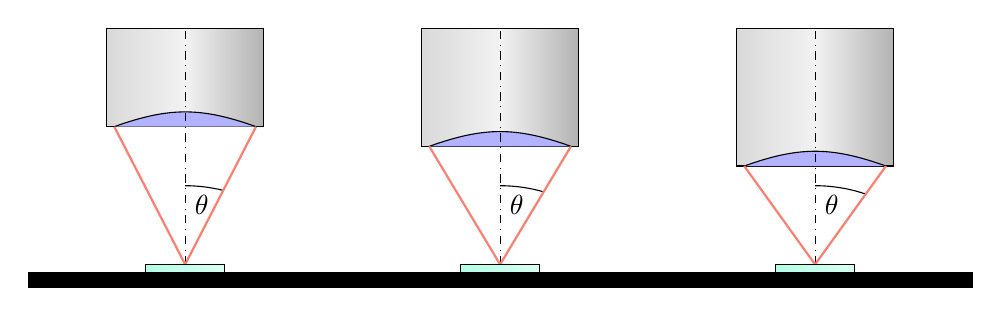
\begin{tikzpicture}
	%primo obiettivo
	\shadedraw[left color=gray!30, right color=gray!60, middle color=gray!10] (1,1.75) -- (1,3) -- (3,3) --(3,1.75) -- cycle;
	\filldraw[blue!30, draw=black] (1.1,1.75)
		.. controls (1.8,2) and (2.2,2)
		.. (2.9,1.75);
	\draw[dash dot] (2,0) -- (2,3);
	\draw (2,1) node[below right]{$\theta$} arc (90:76:2);
	\draw[Salmon, thick] (1.1,1.75) -- (2,0) -- (2.9,1.75);
	\shadedraw[left color=Aquamarine!60, right color=Aquamarine!30] (1.5,0) rectangle (2.5,-0.1);

	%secondo obiettivo
	\shadedraw[left color=gray!30, right color=gray!60, middle color=gray!10] (5,1.5) -- (5,3) -- (7,3) --(7,1.5) -- cycle;
	\filldraw[blue!30, draw=black] (5.1,1.5)
	.. controls (5.8,1.75) and (6.2,1.75)
	.. (6.9,1.5);
	\draw[dash dot] (6,0) -- (6,3);
	\draw (6,1) node[below right]{$\theta$} arc (90:74:2);
	\draw[Salmon, thick] (5.1,1.5) -- (6,0) -- (6.9,1.5);
	\shadedraw[left color=Aquamarine!60, right color=Aquamarine!30] (5.5,0) rectangle (6.5,-0.1);

	%terzo obiettivo
	\shadedraw[left color=gray!30, right color=gray!60, middle color=gray!10] (9,1.25) -- (9,3) -- (11,3) --(11,1.25) -- cycle;
	\filldraw[blue!30, draw=black] (9.1,1.25)
	.. controls (9.8,1.5) and (10.2,1.5)
	.. (10.9,1.25);
	\draw[dash dot] (10,0) -- (10,3);
	\draw (10,1) node[below right]{$\theta$} arc (90:71:2);
	\draw[Salmon, thick] (9.1,1.25) -- (10,0) -- (10.9,1.25);
	\shadedraw[left color=Aquamarine!60, right color=Aquamarine!30] (9.5,0) rectangle (10.5,-0.1);

	%base
	\fill[black] (0,-0.1) rectangle (12,-0.3);
\end{tikzpicture}
\caption{Obiettivi con diverse aperture}
\label{fig:na_diag}
\end{figure}

Per migliorare il potere risolutivo oltre il limite dei $250$ nm, per le lunghezze d'onda dello spettro visibile, si possono usare onde elettromagnetiche con lunghezza minore, come i raggi $X$ o i raggi ultravioletti, oppure raggi di altra natura, come i fasci di elettroni. Queste tecniche portano a risoluzioni maggiori ma presentano anche delle criticità, come una scarsa risposta da parte del campione oppure tossicità.\cite{hell_2007}

\section{Microscopio elettronico}

La scoperta che i raggi di elettroni si comportano come onde con lunghezze d'onda molto più corte della luce visibile aprì nuove possibilità per l'osservazione dei dettagli microscopici. I primi prototipi di microscopi lettronici furono realizzati da \textit{Max Knoll} e \textit{Ernst Ruska}\cite{oatley1982early} e già nel 1933 furono in grado di osservare strutture oltre il limite imposto dai microscopi ottici tradizionali.\cite{physics_nobel}

I microscopi elettronici utilizzano un fascio di elettroni al posto della luce e delle lenti magnetiche al posto delle lenti ottiche. Usando raggi di elettroni invece che di luce, questi microscopi non misurano l'interazione tra materia e luce ma tra materia ed elettroni, aprendo le porte a nuovi campi di studio.

Il campione da esaminare è posto tra il cannone elettronico e il rilevatore e l'immagine si forma in base a come gli elettroni vengono trasmessi attraverso il campione, che deve essere molto sottile (meno di $100$ nm). Questo tipo di microscopi si chiama microscopio elettronico \textit{a trasmissione} (\acrlong{tem} --- \acrshort{tem}) e i modelli più recenti possono arrivare a risoluzioni spaziali fino a $0.5$ \AA\ ($50$ pm).\cite{rolf_2009}

Un altro tipo di microscopio elettronico è quello \textit{a scansione} (\acrlong{sem} --- \acrshort{sem}), in cui non si rileva il fascio trasmesso attraverso il campione, bensì i raggi secondari che sono generati dall'interazione del fascio con il campione (come elettroni secondari o raggi X). Questa tecnica può generare immagini tridimensionali e non richiede un campione sottile quanto la \acrshort{tem}. Modelli recenti di \acrshort{sem} possono arrivare a risoluzioni spaziali fino a $0.4$ nm.\cite{hitachi_sem}\bigskip

\begin{figure}[h]
\centering
\begin{subfigure}[t]{4.5cm}
	\centering
	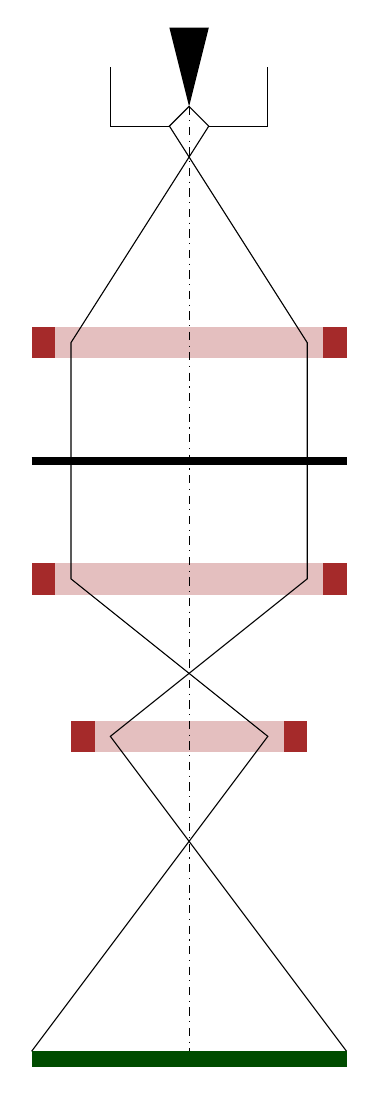
\begin{tikzpicture}
		%cannone
		\fill (1.75,1) -- (2,0) -- (2.25,1) -- cycle;
		\draw (1,0.5) -- (1,-0.25) -- (1.75,-0.25);
		\draw (3,0.5) -- (3,-0.25) -- (2.25,-0.25);

		% condensatore
		\fill[Brown] (0.3,-3.2) rectangle (0,-2.8);
		\fill[Brown] (3.7,-3.2) rectangle (4,-2.8);
		\fill[Brown!30] (0.3,-3.2) rectangle (3.7,-2.8);

		%obiettivo
		\fill[Brown] (0.3,-6.2) rectangle (0,-5.8);
		\fill[Brown] (3.7,-6.2) rectangle (4,-5.8);
		\fill[Brown!30] (0.3,-6.2) rectangle (3.7,-5.8);

		%proiettore
		\fill[Brown] (0.8,-8.2) rectangle (0.5,-7.8);
		\fill[Brown] (3.2,-8.2) rectangle (3.5,-7.8);
		\fill[Brown!30] (0.8,-8.2) rectangle (3.2,-7.8);

		\draw (2,0) -- (1.75,-0.25) -- (3.5,-3) -- (3.5,-6) -- (1,-8) -- (4,-12);
		\draw (2,0) -- (2.25,-0.25) -- (0.5,-3) -- (0.5,-6) -- (3,-8) -- (0,-12);

		\draw[line width=1mm] (0,-4.5) -- (4,-4.5);

		\draw[dash dot] (2,0) -- (2,-12);
		\fill[Green!60!Black] (0,-12) rectangle (4,-12.2);
	\end{tikzpicture}
	\caption{TEM}
\end{subfigure}
\hfill
\begin{minipage}[t]{0.3\textwidth}
	\centering
	\vspace{-12.4cm} Cannone elettronico\\
	\vspace{2.6cm} Lente condensatore\\
	\vspace{1.05cm} Campione\\
	\vspace{1.05cm} Lente obiettivo\\
	\vspace{0.525cm} Bobina di scansione\\
	\vspace{0.525cm} Lente proiettore\\
	\vspace{2cm} Campione\\
	\vspace{1.05cm} Camera CCD\\
\end{minipage}%
\begin{subfigure}[t]{5cm}
	\centering
	\begin{tikzpicture}
		%cannone
		\fill (1.75,1) -- (2,0) -- (2.25,1) -- cycle;
		\draw (1,0.5) -- (1,-0.25) -- (1.75,-0.25);
		\draw (3,0.5) -- (3,-0.25) -- (2.25,-0.25);

		% condensatore
		\fill[Brown] (0.3,-3.2) rectangle (0,-2.8);
		\fill[Brown] (3.7,-3.2) rectangle (4,-2.8);
		\fill[Brown!30] (0.3,-3.2) rectangle (3.7,-2.8);

		% deflettore
		\fill[Blue] (1.7,-6.2) rectangle (1.4,-5.8);
		\fill[Blue] (2.3,-6.2) rectangle (2.6,-5.8);
		\fill[Blue!30] (1.7,-6.2) rectangle (2.3,-5.8);

		%proiettore
		\fill[Brown] (0.8,-8.2) rectangle (0.5,-7.8);
		\fill[Brown] (3.2,-8.2) rectangle (3.5,-7.8);
		\fill[Brown!30] (0.8,-8.2) rectangle (3.2,-7.8);

		%campione
		\draw (2.5,-9.6) -- (1.2,-10) -- (2,-11.2) -- (3.3,-10.8) -- cycle;
		\coordinate (A) at (2.5,-9.6);
		\coordinate (B) at (1.2,-10);
		\coordinate (C) at (2,-11.2);
		\coordinate (D) at (3.3,-10.8);
		\foreach \t in {0.125,0.25,...,0.875} {
			\path
        		coordinate (L) at ($(B)!\t!(A)$)
				coordinate (R) at ($(C)!\t!(D)$);
			\draw[red, dashed, ->] (L) -- (R);
		};

		\draw (2,0) -- (1.75,-0.25) -- (3.5,-3) -- (1,-8) -- (2,-10);
		\draw (2,0) -- (2.25,-0.25) -- (0.5,-3) -- (3,-8) -- (2,-10);

		%indicazioni
		\draw (1.5,-6) -- (-0.5,-7.1);

		\draw[dash dot] (2,0) -- (2,-10);
		\fill[transparent] (0,-12.2){};
	\end{tikzpicture}
	\caption{SEM}
\end{subfigure}%
\caption[Principio di funzionamento dei microscopi TEM e SEM] {
	Principio di funzionamento dei microscopi \acrshort{tem} e \acrshort{sem} }
\label{fig:em_diag}
\end{figure}


Una limitazione di questi tipi di microscopi è che il campione deve essere conduttivo, altrimenti gli elettroni si accumulano sulla superficie del campione e lo caricano, distorcendo l'immagine. Per questo motivo, i campioni non conduttivi devono essere rivestiti con uno strato di metallo (come oro o carbonio) per permettere la conduzione degli elettroni.

\section{Microscopio a effetto tunnel}

La microscopia a scansione di sonda (\acrshort{spm}) fu sviluppata nel 1981 con l'invenzione del microscopio a effetto tunnel (\acrshort{stm}).\cite{ieee_spm}
Questo tipo di microscopi rileva la superficie del campione usando una minuscola punta su cui è imposta una differenza di potenziale con il piano di osservazione. Mantenendo l'altezza della punta costante, si può misurare direttamente la variazione di corrente attraverso il campione in movimento, mentre per misurarne l'altezza si può mantenere costante la corrente e applicare un feedback al motore piezoelettrico che regola l'altezza della punta. Avendo una risoluzione di $0.1$ nm, questa tecnica permette di osservare singoli atomi, ma può essere usata solo se il campione è conduttivo.\cite{bai_2000}

\begin{figure}[h]
\centering
\begin{tikzpicture}
	% punta
	\filldraw[fill=gray] (-0.25,0) -- (-0.25,-1.75) -- (0,-2.5) -- (0.25,-1.75)
		node[right, xshift=3mm] {Punta}
		-- (0.25,0);

	% sistema di controllo
	\fill (-2.5,-1.9) rectangle (-2.45,-1.6);
	\fill (-2.4,-2.1) rectangle (-2.35,-1.4);
	\fill (-2.3,-1.9) rectangle (-2.25,-1.6);
	\fill (-2.2,-2.1) rectangle (-2.15,-1.4);
	\fill (-2.1,-1.9) rectangle (-2.05,-1.6);
	\fill (-2.0,-2.1) rectangle (-1.95,-1.4);
	\draw (-1.95,-1.75) node[above right] {\textbf{+}}
		-- (-0.25,-1.75);
	\draw (-2.5,-3.6) -- (-3,-3.6) -- (-3,-1.75) -- (-2.5,-1.75);
	\draw (-3,-2.75) -- (-5,-2.75) -- (-5, 0);
	\filldraw[fill=white] (-3,-2.75) circle (0.33)
		node[below left, xshift=-3mm, yshift=-3mm] {Amperometro};
	\draw[->] (-3.15,-2.9) -- (-2.85,-2.6);
	\draw[->] (-5,0) -- (-1,0);
	\node[draw, fill=white, align=center] at (-5,0) {Elettronica\\di controllo};

	% cilindro
	\node[cylinder, minimum height=2.5cm, minimum width=2cm, rotate=90, draw,
		shading=axis, left color=gray!30, right color=gray!60, middle color=gray!10] {};
	\filldraw[fill=white] (0,1.225) ellipse (1cm and 0.12cm)
		node[right, xshift=13mm] {Scanner};

	\draw[<->, thick] (1,1.5) -- (-1,1.5) node[midway, above] {X,Y};

	\draw (1,0)
		node[right, xshift=3mm] {Motore piezoelettrico}
		.. controls (1,-0.2) and (-1,-0.2) .. (-1,0);

	\draw[<->, thick] (0,-0.2) -- (0,-1.1) node[midway, right] {Z};

	% campione
	\filldraw[fill=purple] (-2,-3.5) -- (-2,-3.25)
		.. controls (-2,-3) and (-1.33,-3) .. (-1.25,-3.25)
		.. controls (-1,-3.3) and (-0.5, -2.9) .. (0.25,-3.25)
		.. controls (0.75,-3.4) and (1,-3.1) .. (1.7,-3.25)
		.. controls (1.8, -3.2) and (1.9, -3) .. (2,-3)
	 	-- (2,-3.5) node[above right, xshift=3mm] {Campione}
	 	-- cycle;

	 %base
	 \fill (-2.5,-3.5) rectangle (2.5,-3.7);

\end{tikzpicture}
\caption{Principio di funzionamento di un microscopio a effetto tunnel}
\label{fig:stm_diag}
\end{figure}

\section{Atomic Force Microscopy}

Una delle tecniche di microscopia che sono state usate per acquisire le immagini trattate in questa tesi è la microscopia a forza atomica (\acrshort{afm}). Questa tecnica è stata sviluppata nel 1986 da \textit{Gerd Binnig} e \textit{Heinrich Rohrer} ed è un altro tipo di tecnica di microscopia \acrshort{spm} che, permettendo di osservare campioni non conduttivi, a differenza della microscopia \acrshort{stm}, ha aperto la strada a nuove applicazioni.\cite{binnig_1986}

I microscopi \acrshort{afm} usano una punta di diametro di circa $10$ nm fissata a un braccio elastico (\textit{cantilever}), che viene fatta scorrere sulla superficie del campione. La dimensione della punta è importante perché influisce sulla risoluzione spaziale dell'immagine, che può essere minore di un nanometro. La fabbricazione di punte con un raggio così piccolo è una delle limitazioni principali della microscopia \acrshort{afm} e il loro spessore minuscolo fa si che possano essere facilmente danneggiate.\\

\begin{figure}[H]
	\centering
	\begin{subfigure}{4cm}
		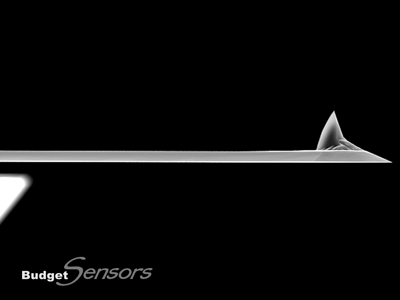
\includegraphics[width=4cm]{images/afm_tip.png}
		\caption{Vista laterale}
	\end{subfigure}
	\hfill
	\begin{subfigure}{4cm}
		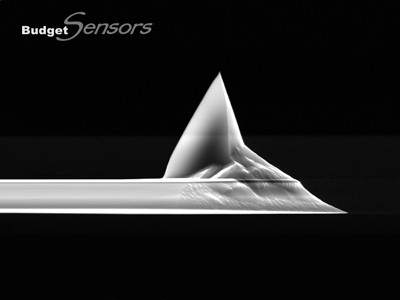
\includegraphics[width=4cm]{images/afm_tip_zoom.png}
		\caption{Vista ingrandita}
	\end{subfigure}
	\hfill
	\begin{subfigure}{4cm}
		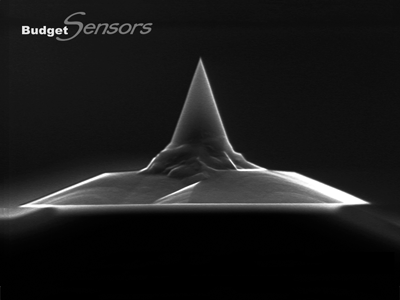
\includegraphics[width=4cm]{images/afm_tip_front.png}
		\caption{Vista frontale}
	\end{subfigure}
\caption[Punta di un microscopio AFM vista al microscopio SEM]{
	Punta di un microscopio \acrshort{afm} vista al microscopio \acrshort{sem}\ \cite{budgetsensors} }
\label{fig:afm_tip}
\end{figure}

Durante la scansione, la punta viene inclinata verso l'alto e il basso a causa della forza di interazione con il campione, che può essere di tipo repulsivo o attrattivo in base alla modalità di scansione. Queste inclinazioni vengono misurate da un raggio laser che viene riflesso dal cantilever su un fotodiodo a quadranti. L'inclinazione del cantilever deflette il raggio laser, che si sposta fra i quadranti del fotodiodo, e il segnale misurato dal fotodiodo viene poi convertito in una variazione di altezza della punta, che viene usata per generare l'immagine del campione.

Per effettuare la scansione, il supporto su cui poggia il campione viene spostato da un sistema piezoelettrico, che può espandersi e contrarsi con una precisione nanometrica applicando una piccola tensione imposta, dell'ordine dei mV. Gli elementi piezoelettrici sono in grado di muoversi in tre direzioni $(X, Y, Z)$ e sono controllati da un sistema elettronico che regola il movimento del campione in modo da mantenere il segnale di riferimento costante.

Con questo sistema si possono apprezzare variazioni di altezza fino a $0.01$ nm.\cite{sun_2018}

\begin{figure}[h]
\centering
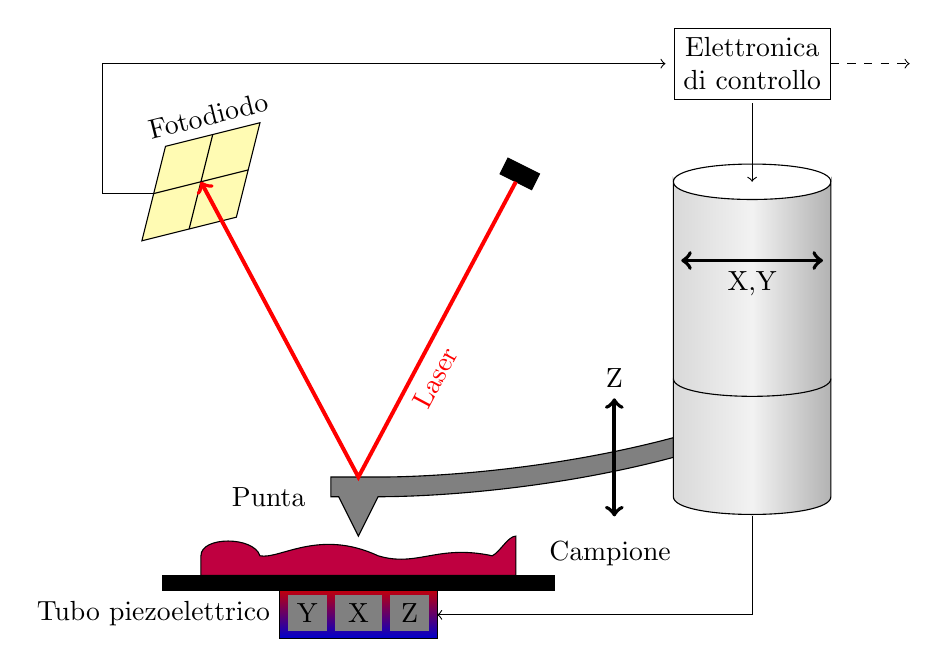
\begin{tikzpicture}
	% punta
	\filldraw[fill=gray] (0.25,-2.25) -- (-0.35,-2.25) -- (-0.35,-2.5)
		-- (-0.25,-2.5) node[left, xshift=-3mm] {Punta}
		-- (0,-3) -- (0.25,-2.5)
		.. controls (1,-2.5) and (2.5, -2.4) .. (4,-2)
		-- (4,-1.75)
		.. controls (2.5, -2.15) and (1,-2.25) .. cycle;

	% campione
	\filldraw[fill=purple] (-2,-3.5) -- (-2,-3.25)
		.. controls (-2,-3) and (-1.33,-3) .. (-1.25,-3.25)
		.. controls (-1,-3.3) and (-0.5, -2.9) .. (0.25,-3.25)
		.. controls (0.75,-3.4) and (1,-3.1) .. (1.7,-3.25)
		.. controls (1.8, -3.2) and (1.9, -3) .. (2,-3)
	 	-- (2,-3.5) node[above right, xshift=3mm] {Campione}
	 	-- cycle;

	%base
	\shadedraw[top color=red!80!black, bottom color=blue!80!black] (-1,-3.65)
		node[below left, yshift=-0.5mm] {Tubo piezoelettrico}
		rectangle (1,-4.3);

	\fill (-2.5,-3.5) rectangle (2.5,-3.7);

	\fill[color=gray] (0.4,-3.75) rectangle (0.9,-4.2) node[midway,black] {Z};
	\fill[color=gray] (-0.4,-3.75) rectangle (-0.9,-4.2) node[midway,black] {Y};
	\fill[color=gray] (-0.3,-3.75) rectangle (0.3,-4.2) node[midway,black] {X};

	% scanner
	\shadedraw[left color=gray!30, right color=gray!60, middle color=gray!10]
		(4,-2.5) .. controls (4,-2.8) and (6,-2.8) .. (6,-2.5)
		-- (6,1.5) .. controls (6,1.2) and (4,1.2) .. (4,1.5)
		-- cycle;
	\draw (6,1.5) .. controls (6,1.8) and (4,1.8) .. (4,1.5);
	\draw (6,-1) .. controls (6,-1.3) and (4,-1.3) .. (4,-1);

	%laser
	\filldraw (1.8,1.6) -- (2.2,1.4) -- (2.3,1.6) -- (1.9,1.8) -- cycle;
	\draw[fill=yellow!30]
		(-2.75,0.75) -- (-2.45, 1.95) -- (-1.25, 2.25)
		node[midway,above,sloped] {Fotodiodo}
		-- (-1.55, 1.05) -- cycle;
	\draw (-2.6,1.35) -- (-1.4,1.65);
	\draw (-2.15, 0.9) -- (-1.85,2.1);
	\draw[line width=0.5mm,red,->] (2,1.5) -- (0,-2.25)
		node[midway,below left,sloped] {Laser}
		-- (-2,1.5);

	% elettronica
	\draw[->] (-2.6,1.35) -- (-3.25,1.35) -- (-3.25,3) -- (3.9,3);
	\draw[dashed,->] (6,3) -- (7,3);
	\node[draw, fill=white, align=center] at (5,3) {Elettronica\\di controllo};
	\draw[->] (5,2.5) -- (5,1.5);
	\draw[->] (5,-2.75) -- (5,-4) -- (1, -4);

	% indicazioni
	\draw[line width=0.5mm,<->] (3.25,-1.25) node[above] {Z}
		-- (3.25,-2.75);

	\draw[line width=0.5mm,<->] (4.1,0.5) -- (5.9,0.5)
		node[below,midway] {X,Y};

\end{tikzpicture}
\caption[Principio di funzionamento di un microscopio AFM]{
	Principio di funzionamento di un microscopio \acrshort{afm}}
\label{fig:afm_diag}
\end{figure}

I microscopi \acrshort{afm} possono essere usati in diverse modalità, a seconda del tipo di interazione che si vuole misurare. Queste modalità possono essere divise in tre categorie principali.\\

\begin{figure}[h]
\centering
\begin{subfigure}{0.32\linewidth}
\centering
	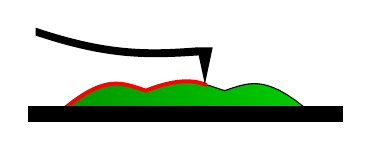
\begin{tikzpicture}
	% campione
	\shadedraw[left color=OliveGreen, right color=green!80!black] (0.5,0)
		.. controls (1, 0.4) and (1.2, 0.3) .. (1.5,0.2)
		.. controls (2,0.4) and (2.2,0.3) .. (2.5,0.2)
		.. controls (2.8, 0.3) and (3, 0.4) .. (3.5,0);
	%solco
	\draw[red, line width=0.5mm, line cap=rect] (0.5,0)
		.. controls (1, 0.4) and (1.2, 0.3) .. (1.5,0.2)
		.. controls (2,0.4) and (2.2,0.29) .. (2.25,0.28);
	%punta
	\fill (2.15,0.75) -- (2.25,0.28) -- (2.35,0.75);
	\fill (2.15,0.75)
		.. controls (1.5,0.7) and (1,0.7) .. (0.1, 1)
		-- (0.1, 0.9)
		.. controls (1,0.6) and (1.5,0.6) .. (2.2,0.65);
	%base
	\fill (0,0) rectangle (4,-0.2);
	\end{tikzpicture}
	\subcaption{Contatto}
	\end{subfigure}
	\begin{subfigure}{0.32\linewidth}
	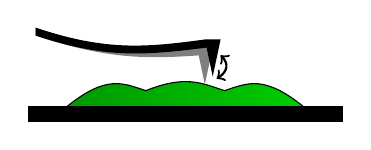
\begin{tikzpicture}
	% campione
	\shadedraw[left color=OliveGreen, right color=green!80!black] (0.5,0)
		.. controls (1, 0.4) and (1.2, 0.3) .. (1.5,0.2)
		.. controls (2,0.4) and (2.2,0.3) .. (2.5,0.2)
		.. controls (2.8, 0.3) and (3, 0.4) .. (3.5,0);
	%punta
	\fill[gray] (2.15,0.75) -- (2.25,0.28) -- (2.35,0.75);
	\fill[gray] (2.15,0.75)
		.. controls (1.5,0.7) and (1,0.7) .. (0.1, 1)
		-- (0.1, 0.9)
		.. controls (1,0.6) and (1.5,0.6) .. (2.2,0.65);
	%punta
	\fill (2.25,0.85) -- (2.35,0.38) -- (2.45,0.85);
	\fill (2.25,0.85)
		.. controls (1.5,0.75) and (1,0.7) .. (0.1, 1)
		-- (0.1, 0.9)
		.. controls (1,0.6) and (1.5,0.65) .. (2.3,0.75);
	%movimento
	\draw[<->, thick] (2.45,0.65) .. controls (2.55,0.55) and (2.55,0.45) .. (2.4,0.35);
	%base
	\fill (0,0) rectangle (4,-0.2);
	\end{tikzpicture}
	\subcaption{Contatto intermittente}
	\end{subfigure}
	\begin{subfigure}{0.32\linewidth}
	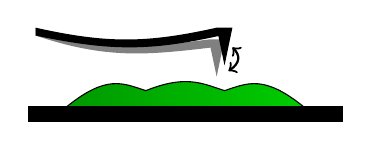
\begin{tikzpicture}
	% campione
	\shadedraw[left color=OliveGreen, right color=green!80!black] (0.5,0)
		.. controls (1, 0.4) and (1.2, 0.3) .. (1.5,0.2)
		.. controls (2,0.4) and (2.2,0.3) .. (2.5,0.2)
		.. controls (2.8, 0.3) and (3, 0.4) .. (3.5,0);
	%punta
	\fill[gray] (2.3,0.85) -- (2.4,0.38) -- (2.5,0.85);
	\fill[gray] (2.3,0.85)
		.. controls (1.5,0.75) and (1,0.7) .. (0.1, 1)
		-- (0.1, 0.9)
		.. controls (1,0.6) and (1.5,0.65) .. (2.35,0.75);
	%punta
	\fill (2.4,1) -- (2.5,0.52) -- (2.6,1);
	\fill (2.4,1)
		.. controls (1.5,0.8) and (1,0.8) .. (0.1, 1)
		-- (0.1, 0.9)
		.. controls (1.05,0.7) and (1.55,0.7) .. (2.45,0.9);
	%movimento
	\draw[<->, thick] (2.6,0.75) .. controls (2.7,0.65) and (2.7,0.55) .. (2.55,0.45);
	%base
	\fill (0,0) rectangle (4,-0.2);
	\end{tikzpicture}
	\subcaption{Senza contatto}
\end{subfigure}
\caption[Modalità di funzionamento di un microscopio AFM]{
	Modalità di funzionamento di un microscopio \acrshort{afm}}
\label{fig:afm_modes}
\end{figure}

\subsection{Modalità a contatto} \label{s:afm_c}

Nella modalità a contatto la forza normale, quindi l'inclinamento verticale del cantilever, è mantenuta costante durante la scansione. Quando la punta si sposta sopra una parte protrudente del campione, il cantilever viene spinto verso l'alto e si crea un errore sull'inclinazione verticale. Per correggere questo errore, il controllore alza la punta finché l'errore non si annulla. Quando si incontrano delle depressioni nel campione si opera il procedimento opposto, abbassando la punta.

Questa modalità permette anche di misurare le forze di attrito tra la superficie del campione e la punta ma non è utilizzabile su campioni biologici perché troppo delicati. La forza esercitata dalla punta può provocare stimoli meccanici non sostenibili per delle cellule e deformare le biomolecole.\cite{zhong_1993}

Idealmente, la forza dovrebbe essere minore di $100$ pN per essere utilizzabile su biomolecole e nell'ordine dei nN per le cellule. Per questo motivo, vengono usati dei cantilever con una bassa costante elastica per diminuire il rumore, aumentare la sensibilità e diminuire la forza di interazione.\cite{wang_2018}

Un altro problema dell'uso di modalità a contatto è la possibilità che cellule poco aderenti o particelle di sporco si attacchino al cantilever.

\subsection{Modalità a contatto infermittente} \label{s:afm_ic}

Nella modalità a contatto intermittente, il cantilever oscilla verticalmente alla sua frequenza di risonanza, o poco meno. Quando la punta scansiona il campione, la sua altezza diminuisce l'ampiezza delle oscillazioni del cantilever che vengono misurate dal fotodiodo. Il segnale di controllo viene regolato in modo che, nel punto più basso del ciclo di oscillazione, la punta tocchi appena il campione. L'ampiezza di queste oscillazioni è quindi una misura delle interazioni tra la punta e il campione. Muovere la punta in alto e in basso, im modo da mantenere la stessa ampiezza di oscillazione, permette di ottenere una topografia del campione.

Altre informazioni che si possono ottenere sono l'ampiezza e la fase dell'errore tra l'oscillazione del cantilever e il segnale di riferimento. Questo scostamento dal segnale di riferimento è causato dalla dissipazione di energia tra la punta e il campione, che può essere dovuta dalle deformazioni della superficie del campione o da forze di attrazione. Queste informazioni possono essere usate per ottenere proprietà viscoelastiche del campione e distinguere materiali diversi.\cite{bruker_phase_imaging}

Al contrario della modalità a contatto, la forza laterale è trascurabile visto che la punta tocca il campione solo per un istante ed è maggiormente indicata per campioni biologici, che altrimenti si muoverebbero liberamente insieme alla punta.\cite{karrasch_1993}

Questa modalità di operazione è più lenta rispetto alla modalità a contatto a causa del meccanismo di scansione. Mentre nella modalità a contatto intermittente il segnale è generato dalla modulazione in ampiezza del cantilever, nella modalità a contatto si usa la deflessione del cantilever, che varia molto più velocemente. Questa differenza si riflette anche nel comportamento del controllore: la modalità a contatto è più stabile ad alti guadagni, che invece possono generare forti artefatti o immagini rumorose nella modalità a contatto intermittente. I parametri del controllore devono quindi essere scelti con più attenzione. 

\subsection{Modalità senza contatto} \label{s:afm_nc}

Nella modalità senza contatto, la punta non tocca mai il campione ma mantiene comunque un'alta sensibilità alla sua topologia. Per fare ciò, la punta deve trovarsi abbastanza vicino al campione da entrare nel suo campo di forze, ma senza passare nella regione attrattiva usata per le modalità a contatto.

Questa scelta comporta l'uso di un cantilever molto rigido che rimane molto vicino alla superficie del campione per osservare come cambiano l'ampiezza e la fase della sua oscillazione, evitando che passi al regime repulsivo. Questi sono effetti della variazione della frequenza di oscillazione in risposta alle forze applicate dalla superficie sulla punta (forze di van der Waals).

Per questa modalità si usa un cantilever ad alta frequenza di risonanza, tipicamente compresa tra $300$ e $400$ kHz, e bassa ampiezza di oscillazione, di circa $10$ nm.\cite{giessibil_1999} Come per la modalità a contatto intermittente, la velocità di scansione è più bassa di quella della modalità a contatto, ma queste proprietà del cantilever permettono di avere velocità maggiori della modalità a contatto intermittente.

Non entrando mai nella regione ripulsiva, questa modalità presenta il più basso rischio di danneggiare o contaminare la punta e il campione.\cite{ho_1996}

\vspace{2mm}

\begin{figure}[h]
\centering
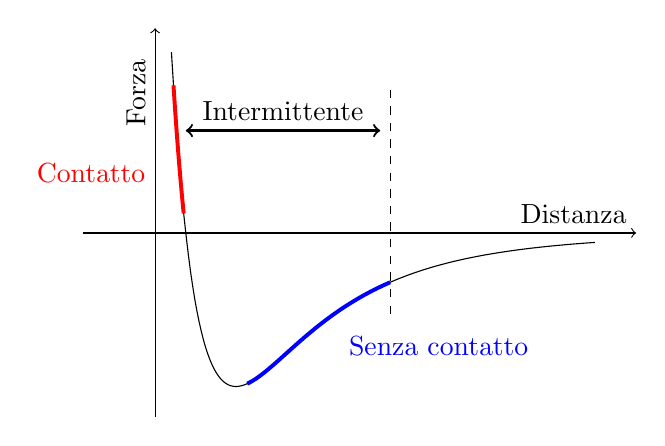
\begin{tikzpicture}[domain=1.93:4, samples=200, scale=2.6]
	%assi
	\draw[->] (1.5,0) -- (4.2,0) node[above left] {Distanza};
	\draw[->] (1.85,-0.9) -- (1.85,1) 
		node[above right,midway,sloped, xshift=11mm] {Forza};
		
	%grafico
	\draw plot (\x,{3*((2/\x)^(12)-(2/\x)^6)});
	
	%regione contatto
	\draw[domain=1.94:1.99, red, line width=0.5mm] plot (\x,{3*((2/\x)^(12)-(2/\x)^6)});
	\node[red,above left] at (1.85,0.2) {Contatto};
	
	%regione senza contatto
	\draw[domain=2.3:3, blue, line width=0.5mm] plot (\x,{3*((2/\x)^(12)-(2/\x)^6)});
	\node[blue,right] at (2.75,-0.55) {Senza contatto};
	
	%regione intermittente
	\draw[dashed] (3,0.7) -- (3,-0.4);
	\draw[<->, thick] (2, 0.5) -- (2.95,0.5)
		node[above,midway] {Intermittente};
\end{tikzpicture}
\caption[Grafico delle forze di van der Waals secondo il modello di Lennard-Jones] {
	\begin{tabular}[t]{ @{} l @{} }
		Grafico delle forze di van der Waals secondo il modello di Lennard-Jones\\
		Semipiano superiore: Forze repulsive\\
		Semipiano inferiore: Forze attrattive
	\end{tabular}}
\label{fig:waals}
\end{figure}

Le modalità descritte nei paragrafi precedenti fanno tipicamente uso della modulazione in ampiezza. L'uso della modulazione in frequenza è limitato in quanto richiede attrezzature specifiche e un ambiente a vuoto ultra spinto. Usare una modalità oscillante a modulazione in frequenza ha anche dei vantaggi, come una risoluzione più alta.\cite{sugawara_1995}

\subsection{Sistema di controllo}

Il controllo del sistema è affidato a un controllore \acrshort{pid} (\acrlong{pid}), di gran lunga il tipo di sistema di controllo più usato (nel 95\% di tutti i casi).\cite{astrom_2010}

\begin{figure}[h]
\centering
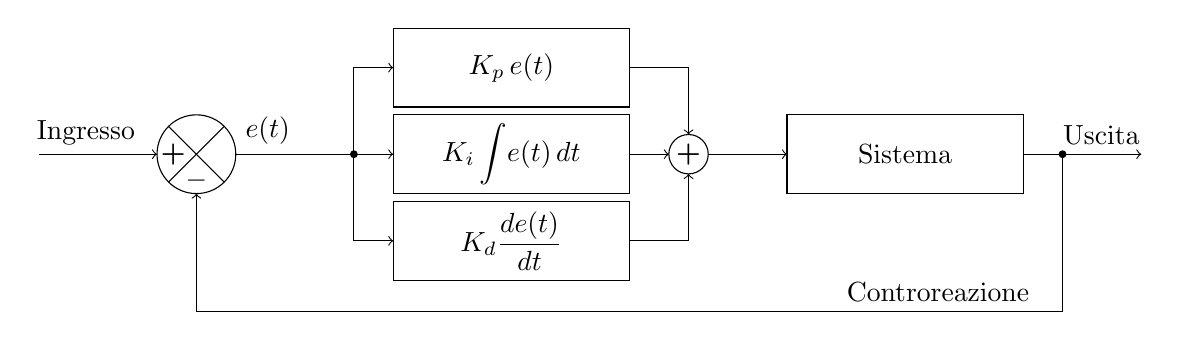
\begin{tikzpicture}
	
	\draw[->] (-2,0) node[above right, xshift=-1.5mm] {Ingresso} 
		-- (-0.5,0) node[right, xshift=-0.75mm] {\textbf{+}};
	
	\draw (0,0) circle (0.5);
	\draw (0.3535,-0.3535) -- (-0.3535,0.3535);
	\draw (-0.3535,-0.3535) -- (0.3535,0.3535);
	
	\draw[->] (0.5,0) node[above right] {$e(t)$} -- (2.5,0);
	\draw[->] (2,0) -- (2,1.1) -- (2.5,1.1);
	\draw[->] (2,0) -- (2,-1.1) -- (2.5,-1.1);
	\fill (2,0) circle (0.05);
	
	\draw[->] (5.5,0) -- (6,0);
	\draw[->] (5.5,1.1) -- (6.25,1.1) -- (6.25,0.25);
	\draw[->] (5.5,-1.1) -- (6.25,-1.1) -- (6.25,-0.25);
	\draw (6.25,0) circle (0.25) node {\textbf{+}};
	
	%controllore
	\draw (2.5,1.6) rectangle (5.5,0.6)
		node[midway] {$\displaystyle K_p\,e(t)$};
	\draw (2.5,0.5) rectangle (5.5,-0.5)
		node[midway] {$\displaystyle K_i\int\!e(t)\,dt$};
	\draw (2.5,-0.6) rectangle (5.5,-1.6)
		node[midway] {$\displaystyle K_d\frac{de(t)}{dt}$};
	
	\draw[->] (6.5,0) -- (7.5,0);
	\draw (7.5,0.5) rectangle (10.5,-0.5)
		node[midway] {Sistema};
	
	\draw[->] (10.5,0) -- (12,0) node[above left, xshift=1mm] {Uscita};
	\draw[->] (11,0) -- (11,-2) node[above left, xshift=-3mm] {Controreazione}
		-- (0,-2) -- (0,-0.5) node[above, yshift=-0.75mm] {$-$};
	\fill (11,0) circle (0.05);
\end{tikzpicture}
\caption[Diagramma di un controllore PID ad anello chiuso] {
	\begin{tabular}[t]{ @{} l @{} }
		Diagramma di un controllore PID ad anello chiuso\\
		$e(t)$: funzione di errore
	\end{tabular}}
\label{fig:pid_diag}
\end{figure}

Quando le forze di interazione tra la punta e il campione cambiano, il cantilever si flette e, di conseguenza, modifica l'uscita del fotodiodo facendola deviare dal valore di ingresso. La differenza tra ingresso e uscita è la funzione di errore $e(t)$.

Il controllore PID agisce su questa funzione e il suo comportamento è composto da tre azioni indipendenti, controllate da altrettante variabili di regolazione.\cite{ogata_2010}
\begin{itemize}
	\itemsep0em 
	\item Il termine \textbf{P} (\textit{azione proporzionale}) è proporzionale alla funzione di errore
	\item Il termine \textbf{I} (\textit{azione integrativa}) è l'integrale dei valori passati di $e(t)$
	\item Il termine \textbf{D} (\textit{azione derivativa}) è una stima delle variazioni future di $e(t)$
\end{itemize}

Il sistema di feedback comprende tre meccanismi principali: \cite{parisi}
\begin{enumerate}
	\itemsep0em 
	\item Il tubo piezoelettrico per il controllo del movimento e della posizione della punta rispetto alla superficie del campione
	\item Il cantilever e il sistema ottico per la misura della distanza tra la sonda e la superficie del campione
	\item Il circuito di controllo per mantenere una deflessione costante correggendo la tensione applicata al tubo piezoelettrico
\end{enumerate}

Per sua natura, un microscopio \acrshort{afm} è molto versatile e presenta molti parametri che si possono regolare per ottimizzare la resa delle immagini. Partendo da quelli più generali, si può impostare una modalità operativa, come quelle descritte sopra (\textit{vedi} \ref{s:afm_c}, \ref{s:afm_ic}, \ref{s:afm_nc}), e un tipo di cantilever che più si adattano al campione scelto.

Passando ai parametri di scansione, si possono impostare la velocità e l'area di scansione controllando opportunamente il sistema piezoelettrico su cui poggia il campione. L'area di scansione rappresenta il campo di osservazione del campione (es. $10$ µm $\times$ $10$ µm) ed influenza la risoluzione delle immagini. La velocità di scansione, espressa in µm/s o linee al secondo (Hz), è inversamente proporzionale alla qualità dell'immagine, ma con basse velocità aumenta il rischio di muovere parti del campione.

È possibile anche regolare dei parametri relativi all'interazione tra la punta e il campione, come l'ampiezza e la frequenza di oscillazione (solo in modalità oscillanti) e la forza di carico desiderata. Per regolare questi parametri si può operare sull'ingresso del sistema e sul guadagno dell'anello di feedback.

\section{Scanning Near-field Optical Microscopy}

L'altra tecnica di microscopia usata per ottenere le immagini studiate in questa tesi è la microscopia ottica a scansione del campo vicino (\acrlong{snom} --- \acrshort{snom}). Questa tecnica riesce a superare il limite di risoluzione sfruttando delle proprietà dei campi evanescenti. Ad \textit{Edward Hutchinson Synge} è attribuito il merito di aver proposto per primo questa tecnica nel 1928,\cite{synge_1928} ma il primo microscopio \acrshort{snom} fu costruito solo nel 1984 da \textit{Dieter Pohl}.\cite{pohl_1984}

I campi evanescenti possono essere descritti da onde piane della forma $\mathbf{E}e^{i(\mathbf{kr}-\omega t)}$, che sono caratterizzate dal fatto che almeno una componente del vettore d'onda \textbf{k}, che descrive la direzione di propagazione, è immaginaria. Nella direzione spaziale definita dalla componente immaginaria, l'onda non si propaga ma decade esponenzialmente. I campi evanescenti sono di grande importanza per lo studio e la comprensione dei campi ottici confinati a dimensioni inferiori alla lunghezza d'onda.\cite{novotny_2012}

Come descritto nel paragrafo \ref{s:na}, un microscopio ottico tradizionale, per ottenere un immagine del campione, deve raccogliere tutta la luce diffratta nel campo lontano, che si propaga senza restrizioni.
Al contrario, la microscopia \acrshort{snom} utilizza un laser la cui luce è concentrata in un'apertura di diametro molto inferiore alla sua lunghezza d'onda, creando un campo evanescente dall'altro lato dell'apertura.\cite{betzig_1992} Quando il campione viene scansionato ad una piccola distanza sotto l'apertura ($<10$ nm), la risoluzione ottica della luce trasmessa o riflessa è limitata solo dal diametro dell'apertura. I campi evanescenti trasportano informazioni ad alte frequenze spaziali sul campione e permettono di arrivare a una risoluzione laterale di $6$ nm\cite{ma_2021} e una risoluzione verticale di $2$ nm.\cite{oshikane_2007}\\

\begin{figure}[h]
	\centering
	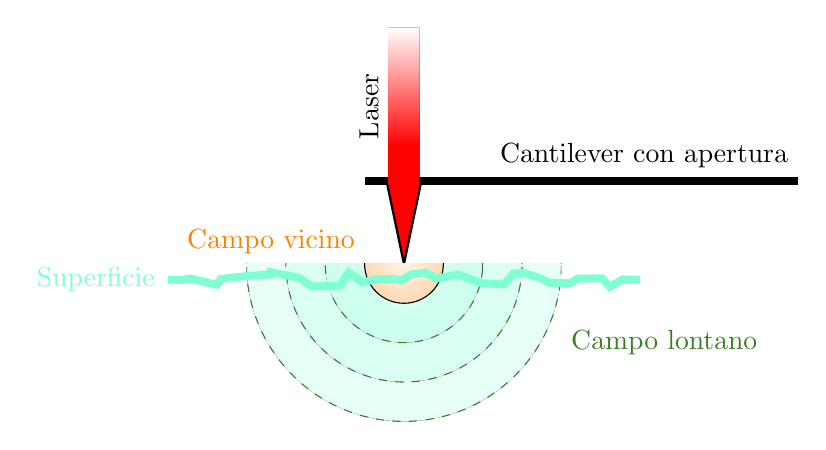
\begin{tikzpicture}
		% cantilever
		\fill (-0.5,1) rectangle (5,1.1);
		\node[above left] at (5,1.1) {Cantilever con apertura};
		
		%laser
		\fill[top color=red!0, bottom color=red, middle color=red] 
			(0.2,3) -- (0.2,1) -- (0,0) -- (-0.2,1) 
			-- (-0.2,3) node[midway, above, sloped] {Laser}
			-- cycle;
			
		%punta
		\draw[thick, line cap=rect]  (-0.21,1) -- (0,0) -- (0.21,1);
		
		%linee di campo
		\begin{scope}
			\clip (-2,0) rectangle (2,-2);
			
			\filldraw[inner color=Aquamarine!10, outer color=Aquamarine!20, dashed, draw=OliveGreen] 
				(0,0) circle (2);
			\filldraw[inner color=Aquamarine!20, outer color=Aquamarine!30, dashed, draw=OliveGreen] 
				(0,0) circle (1.5);
			\filldraw[inner color=Aquamarine!30, outer color=Aquamarine!40, dashed, draw=OliveGreen] 
				(0,0) circle (1);
			\filldraw[inner color=orange!10, outer color=orange!30] (0,0) circle (0.5);
		\end{scope}
		
		\node[above left, orange] at (-0.5,0) {Campo vicino};
		\node[right, OliveGreen] at (2,-1) {Campo lontano};
		
		%superficie campione
		\draw[Aquamarine, line width=1mm, decorate, decoration={random steps,segment length=5pt,amplitude=3pt}] 
			(-3,-0.2) node[left] {Superficie}
			-- (3,-0.2);
	\end{tikzpicture}
	\caption[Principio di funzionamento di un microscopio SNOM]{
		Principio di funzionamento di un microscopio \acrshort{snom}}
	\label{fig:asnom_diag}
\end{figure}

Poiché le onde evanescenti sono confinate a una regione prossima alla superficie del mezzo che le origina, è necessario portare il rilevatore entro l'intervallo della lunghezza d'onda della radiazione utilizzata. Su queste onde si applica il \textit{principio di reciprocità di Helmholtz}, secondo cui il campo vicino può essere convertito in onde propaganti dal rilevatore. Grazie a questo principio, i raggi entranti e uscenti possono essere considerati uno come il reciproco dell'altro, permettendo di usare la sonda ottica sia come sorgente che come rilevatore.\cite{hapke_1993}

Per questo motivo, una delle limitazioni principali di questa tecnica è la distanza di lavoro molto breve e una profondità di campo estremamente ridotta. Normalmente questi microscopi sono usati per studi di superficie, ma si possono anche usare per studiare regioni di interesse sotto la superficie, posto che siano entro il limite della profondità di campo.\cite{vobornik_2008}

\subsection{Aperture SNOM}

Nella microscopia \acrshort{asnom} la sonda ottica è installata nella punta, che ha un foro di dimensioni minori della lunghezza d'onda del raggio, da cui la luce può essere emessa o ricevuta. La luce è condotta alla punta da un cavo in fibra ottica monomodale e la punta ha uno strato metallico di rivestimento per riflettere i raggi. La dimensione dell'apertura può arrivare fino a circa $50$ nm e influenza la risoluzione spaziale delle immagini.\cite{antosiewicz_2011}

\begin{figure}[h]
\centering
\begin{subfigure}{0.35\linewidth}
	\centering
	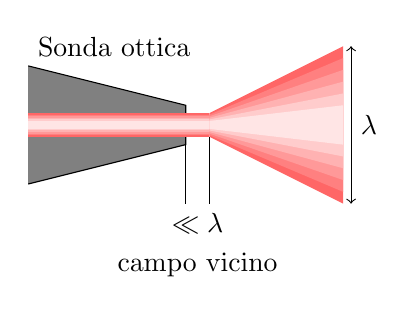
\begin{tikzpicture}
		%sonda
		\filldraw[fill=gray] (-2,0.75) node[above right] {Sonda ottica} 
			-- (0,0.25) -- (0,-0.25) -- (-2,-0.75);
		
		%luce nella sonda
		\fill[red!60] (-2,0.15) rectangle (0.3,-0.15);
		\fill[red!50] (-2,0.13) rectangle (0.3,-0.13);
		\fill[red!40] (-2,0.11) rectangle (0.3,-0.11);
		\fill[red!30] (-2,0.09) rectangle (0.3,-0.09);
		\fill[red!20] (-2,0.07) rectangle (0.3,-0.07);
		\fill[red!10] (-2,0.05) rectangle (0.3,-0.05);
		
		%luce fuori sonda
		\fill[red!60] (0.3,-0.15) -- (2,-1) -- (2,1) -- (0.3,0.15) -- cycle;
		\fill[red!50] (0.3,-0.13) -- (2,-0.85) -- (2,0.85) -- (0.3,0.13) -- cycle;
		\fill[red!40] (0.3,-0.11) -- (2,-0.70) -- (2,0.70) -- (0.3,0.11) -- cycle;
		\fill[red!30] (0.3,-0.09) -- (2,-0.55) -- (2,0.55) -- (0.3,0.09) -- cycle;
		\fill[red!20] (0.3,-0.07) -- (2,-0.40) -- (2,0.40) -- (0.3,0.07) -- cycle;
		\fill[red!10] (0.3,-0.05) -- (2,-0.25) -- (2,0.25) -- (0.3,0.05) -- cycle;
		
		\draw (0,-0.25) -- (0,-1);
		\draw (0.3,-0.15) -- (0.3,-1);
		
		\node[below] at (0.15,-1) {$\ll\lambda$};
		\node[below] at (0.15, -1.5) {campo vicino};
		\draw (0,-0.25) -- (0,-1);
		
		\draw[<->] (2.1,-1) -- (2.1,1) node[right,midway] {$\lambda$};
	\end{tikzpicture}
\subcaption{Schema}
\end{subfigure}
\begin{subfigure}{0.3 \linewidth}
	\centering
	\raisebox{0.5cm}{
	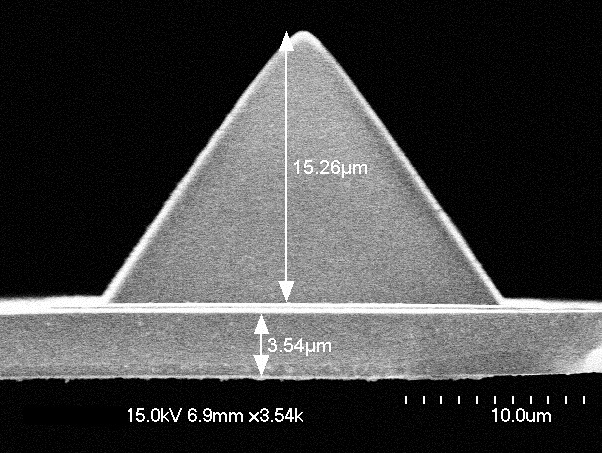
\includegraphics[keepaspectratio, width=3cm]{images/snom_tip.jpeg}}
	\subcaption{Punta reale \cite{tipsnano} }
\end{subfigure}
\begin{subfigure}{0.3 \linewidth}
	\centering
	\raisebox{0.25cm}{
	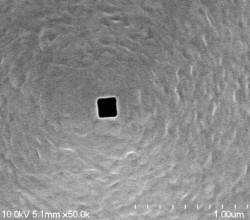
\includegraphics[keepaspectratio, width=3cm]{images/snom_tip_front.jpeg}}
	\subcaption{Vista sul foro}
\end{subfigure}
\caption[Ingrandimento sull'apertura della punta in un microscopio a-SNOM]{
	Ingrandimento sull'apertura della punta in un microscopio \acrshort{asnom}}
\label{fig:snom_probe}
\end{figure}

La maggior parte dei microscopi \acrshort{asnom} usa un metodo simile a quello dei microscopi \acrshort{afm} senza contatto (\textit{vedi} \ref{s:afm_nc}) basato sulla forza di taglio per controllare la distanza tra la punta e il campione. La sonda è messa in vibrazione alla sua frequenza di risonanza parallelamente alla superficie con un'ampiezza minore di $5$ nm. L'ampiezza e la fase di queste oscillazioni della fibra sono monitorate da un apposito sensore di spostamento.\cite{hecht_2000}

\subsubsection{Modalità di operazione}

I microscopi \acrshort{asnom} possono operare secondo diverse modalità, che dipendono principalmente dal percorso che compie la luce. Nella modalità più utilizzata la punta è usata sia per illuminare il campione che per raccogliere la luce generata nel campo vicino.\cite{alvarez_2006}\\

\begin{figure}[h]
	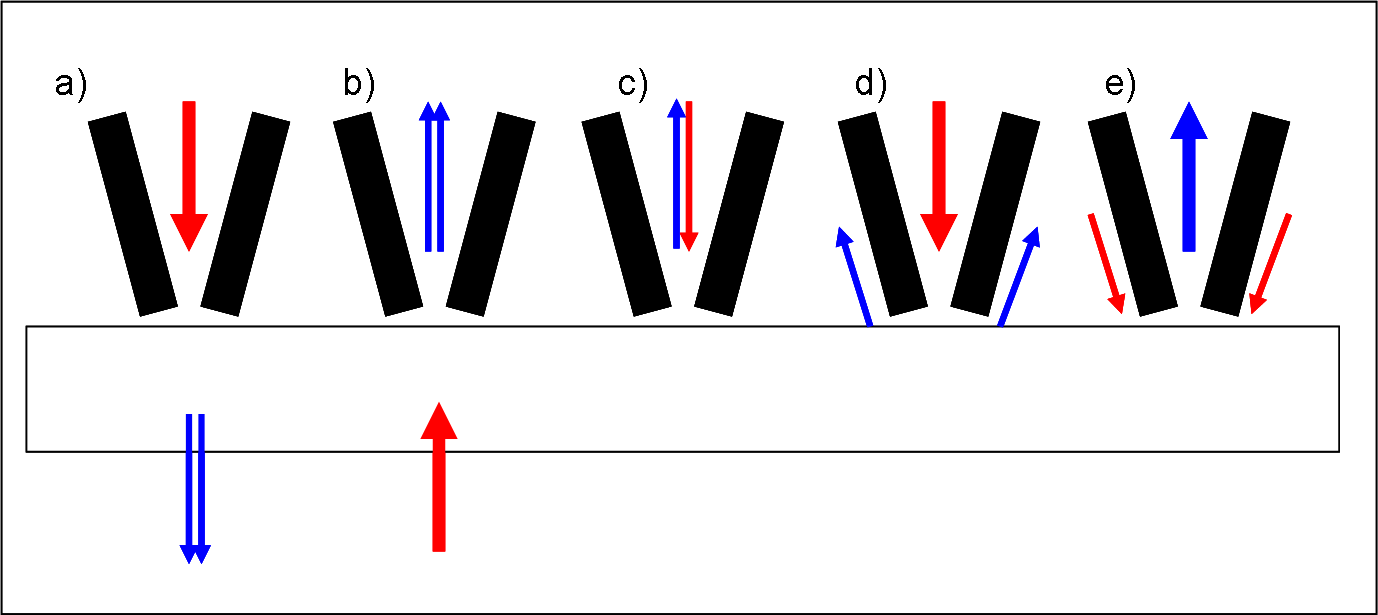
\includegraphics[keepaspectratio, width=\linewidth]{images/snom_apertures.png}
	\caption[Modalità di illuminazione di un microscopio a-SNOM]{
		Modalità di illuminazione di un microscopio \acrshort{asnom}}
	\label{fig:snom_apertures}
\end{figure}

\begin{enumerate}[a)]
	\item In questa configurazione, la luce viene emessa da un laser e trasmessa alla punta dal cavo in fibra ottica. L'apertura estremamente ristretta della punta crea un campo evanescente sulla superficie del campione. Questo campo poi interagisce con il campione e la radiazione convertita viene diffusa e raccolta da un obiettivo ottico convenzionale nel campo lontano.
	\item Al contrario della modalità di illuminazione, il campione è illuminato esternamente con luce dal campo lontano (ad esempio un laser o una lampada), mentre la punta viene usata come un rivelatore. Le onde evanescenti sulla superficie del campione vengono convertite in onde propaganti dentro la punta e trasmesse al rilevatore.
	\item In questo caso, la punta illumina il campione e riceve anche la luce riflessa. Sia l'emissione che la raccolta avvengono attraverso la stessa apertura. In questo caso è necessario installare un dispositivo che separi i due flussi di luce.
	\item[d-e)] Queste modalità sono simili alle prime, con la differenza che si basano sulla luce riflessa per effettuare le misure.
\end{enumerate}

\subsection{Apertureless SNOM}

La struttura di un microscopio \textit{apertureless SNOM}, anche detto di tipo scattering (\acrshort{ssnom}),  è molto simile a quella di un microscopio \acrshort{afm}, in quanto sono entrambe tecniche di microscopia \acrshort{spm}, e per questo lo stesso macchinario può offrire entrambe le tecniche di acquisizione. Questi sistemi possono anche essere combinati con altre tecniche di imaging, come la spettroscopia Raman\cite{zhang_2017} o la spettroscopia infrarossa a trasformata di Fourier (\acrshort{ftir}) \cite{rotenberg_2014}.

In questo caso si utilizza una punta metallica o rivestita in metallo per sondare il campo elettrico locale vicino al campione. Con una fonte di luce esterna a una frequenza a scelta, la punta metallica sparge la luce in base alla sua polarizzabilità. La presenza del campione sotto la punta metallica modifica la polarizzabilità della punta in funzione della costante dielettrica del campione. Scansionando la punta metallica sulla superficie del campione con un microscopio \acrshort{afm} in modalità a contatto intermittente (\textit{vedi} \ref{s:afm_ic}) si ottiene il segnale usato per formare l'immagine contenente informazioni sulle proprietà ottiche del campione.\cite{wang_2015}

I modelli numerici per lo studio delle interazioni nel campo vicino tra la punta e la superficie del campione usano tecniche di elaborazione diverse, come il modello a dipolo puntiforme e a dipolo finito.\cite{cvitkovic_2007}\\

\begin{figure}[h]
\begin{subfigure}{0.5\linewidth}
	\centering
	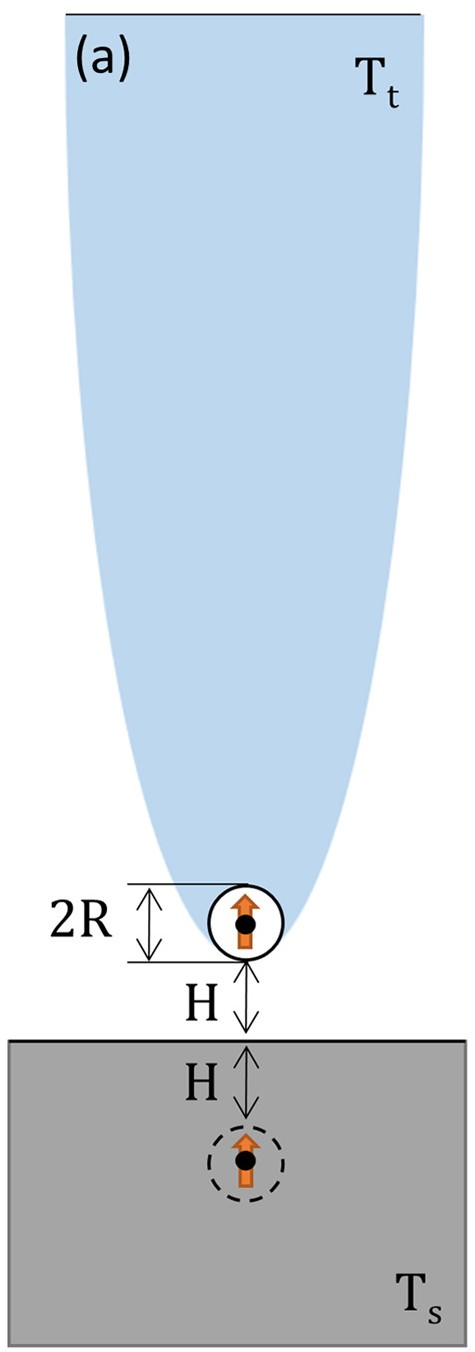
\includegraphics[keepaspectratio, height=\linewidth]{images/pdm.jpeg}
	\subcaption{Point Dipole Model}
\end{subfigure}
\begin{subfigure}{0.5\linewidth}
	\centering
	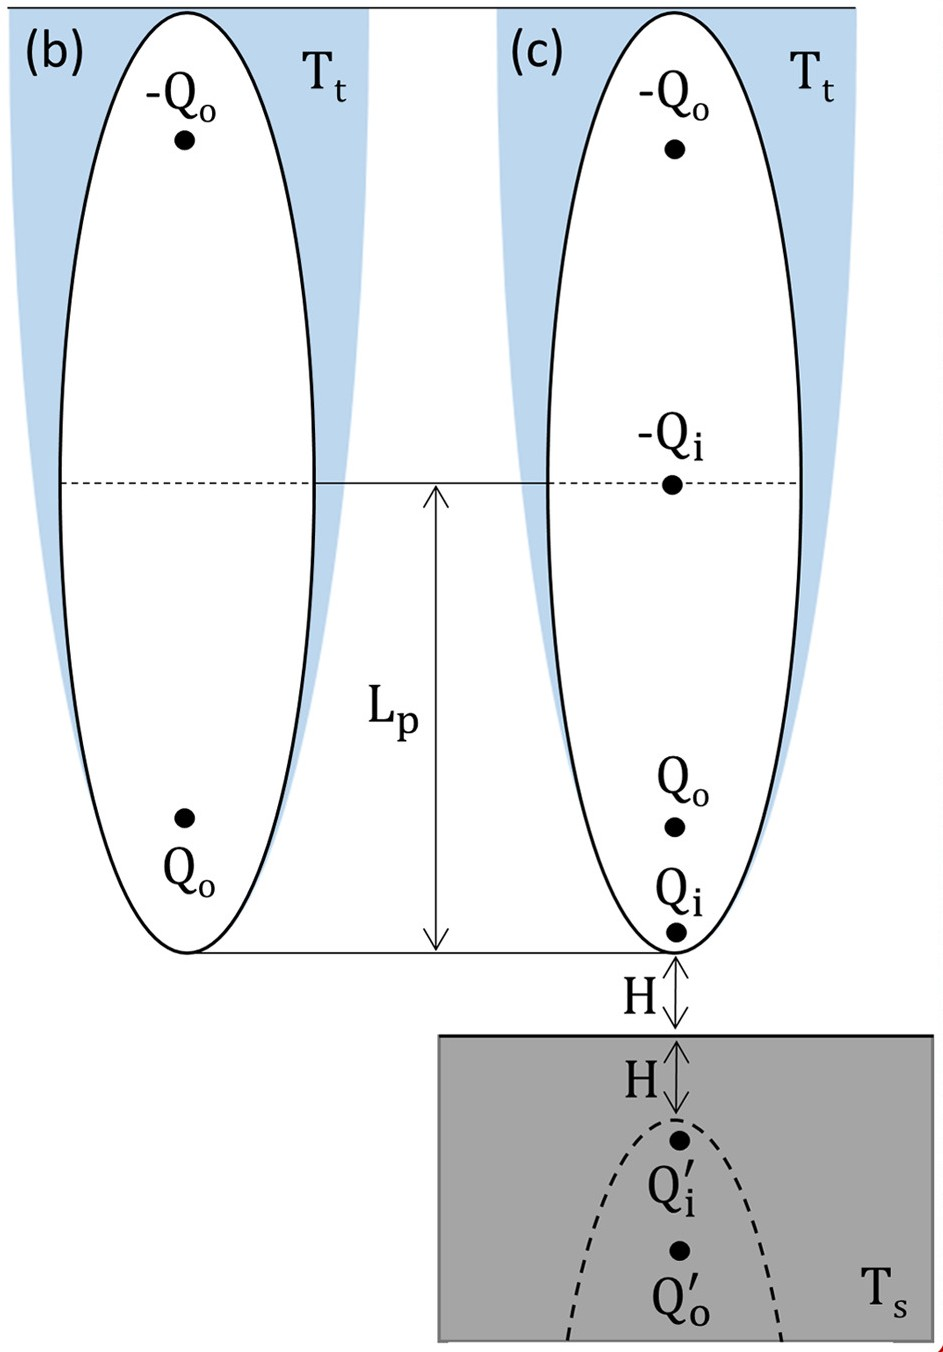
\includegraphics[keepaspectratio, height=\linewidth]{images/fdm.jpeg}
	\subcaption{Finite Dipole Model}
\end{subfigure}
\caption{Modelli di dipoli usati per elaborare le radiazioni nel campo vicino}
\label{fig:dipole_model}
\end{figure}

Nel modello a dipolo puntiforme la punta della sonda è modellizzata come un punto con un certo momento di dipolo \textbf{p} generato dal campo elettrico incidente $\mathbf{E}$. Il momento del dipolo è, quindi
\begin{equation}
	\mathbf{p}=\alpha\mathbf{E}
\end{equation}
dove $\alpha$ è il tensore di polarizzabilità della punta. Il campione genera un dipolo immagine che modifica il campo elettrico locale percepito dalla punta. La misurazione viene effettuata sulla radiazione prodotta da questo dipolo indotto. Questa approssimazione è buona per studi qualitativi ma ignora la geometria reale della punta e non tiene conto della distribuzione delle cariche lungo essa.\cite{wu_2005}

Nel modello a dipolo finito la punta è rappresentata come un oggetto esteso, come uno sferoide. Il momento di dipolo non è quindi localizzato in un solo punto, ma è distribuito lungo l'asse. Questo modello è più accurato, specialmente per punte lunghe, e tiene conto delle risonanze plasmoniche lungo la punta.\cite{jarzembski_2017}

La rilevazione del segnale è effettuata da un interferometro di Michelson, con la particolarità che uno degli specchi è mobile. Questa tecnica di misura prende il nome di spettroscopia a trasformata di Fourier (\acrshort{fts}). Il segnale viene registrato mentre lo specchio è in movimento, creando un interferogramma, e poi convertito in uno spettro dalla trasformata.\cite{moreno_2017}

\begin{figure}[ht]
\centering
\begin{tikzpicture}

	%beam splitter
	\filldraw[upper left=gray, lower right=gray] (-0.75,-0.75) rectangle (0.75,0.75);
	\draw (-0.75,0.75) -- (0.75,-0.75) node[below right] {Beam-splitter};

	%laser
	\fill (-3.5,-0.25) rectangle (-2.5,0.25);
	\draw[-{Latex}, line width=1mm, red] (-2.5,0) -- (0,0);
	\node[above] at (-3,0.25) {Laser};
	
	%specchio riferimento
	\draw[{Latex}-{Latex}, line width=1mm, red] (0,-2) -- (0,0);
	\filldraw[left color=Aquamarine!60, right color=Aquamarine!30] (-1,-2) rectangle (1,-2.2)
		node[right, yshift=0.5mm] {Specchio};
	\draw[<->] (-1.3,-1.8) -- (-1.3,-2.4) 
		node[midway, left, xshift=-1.75mm] {$\phi_c\cos\left(\omega_c t\right)$};
		
	%rilevatore
	\draw[{Latex}-, line width=1mm, red] (0,2) -- (0,0);
	\filldraw[fill=gray]  (-1,2) rectangle (1,2.2)
		node[right, yshift=-1mm] {Rilevatore};
	
	%obiettivo
	
	\draw[line width=1.5mm]	(6,0.6) .. controls (6.65,0.6) and (7.75,-0) .. (7.75,-0.75);
	\draw[{Latex}-{Latex},red, line width=0.5mm] (0,0) -- (7.3,0);
	\draw[{Latex}-{Latex},red, line width=0.5mm] (7.3,0) -- (6.1,-1.75);
	
	\begin{scope}[ shift={(3.75,-2.05)}]
	% campione
		\shadedraw[left color=OliveGreen, right color=green!80!black] (0.5,0)
		.. controls (1, 0.4) and (1.2, 0.3) .. (1.5,0.2)
		.. controls (2,0.4) and (2.2,0.3) .. (2.5,0.2)
		.. controls (2.8, 0.3) and (3, 0.4) .. (3.5,0);
		%punta
		\fill (2.15,0.75) -- (2.25,0.28) -- (2.35,0.75);
		\fill (2.15,0.75)
		.. controls (1.5,0.7) and (1,0.7) .. (0.1, 1)
		-- (0.1, 0.9)
		.. controls (1,0.6) and (1.5,0.6) .. (2.2,0.65);
		%base
		\fill (0,0) rectangle (4,-0.2);
	\end{scope}

\end{tikzpicture}
\caption[Sistema di rilevazione a pseudo-eterodina per microscopia s-SNOM]{
	Sistema di rilevazione a pseudo-eterodina per microscopia \acrshort{ssnom}}
\end{figure}

\end{document}
  